\documentclass[border=6pt]{standalone}
\usepackage{tikz}
\usetikzlibrary{arrows.meta}
\begin{document}
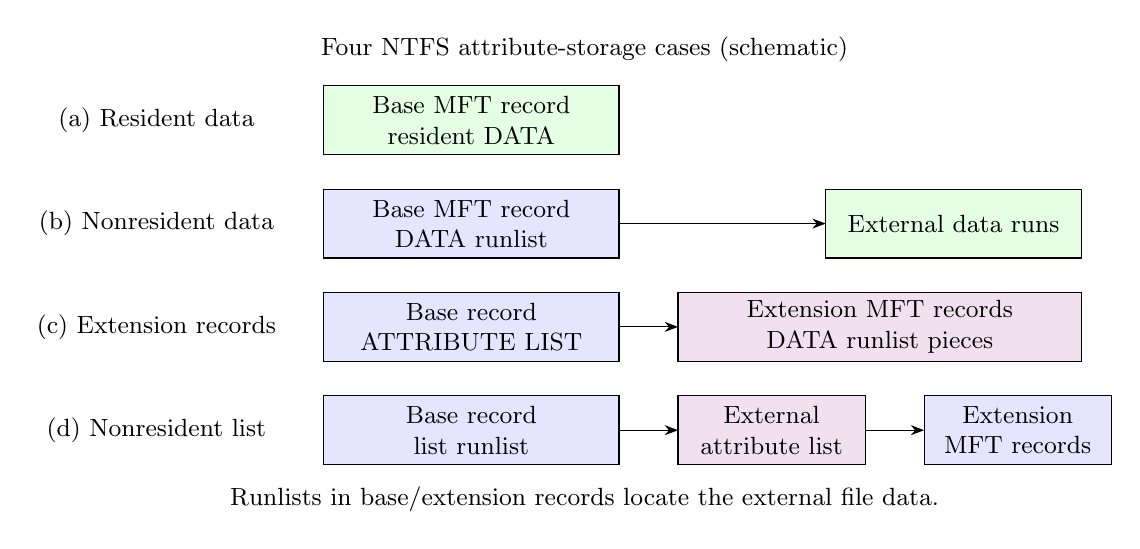
\begin{tikzpicture}[>=Stealth]
\node[align=center,font=\small] at (7.188,6.025) {Four NTFS attribute-storage cases (schematic)};
\node[align=center,font=\small] at (1.750,5.125) {(a) Resident data};
\node[align=center,font=\small] at (1.750,3.812) {(b) Nonresident data};
\node[align=center,font=\small] at (1.750,2.500) {(c) Extension records};
\node[align=center,font=\small] at (1.750,1.188) {(d) Nonresident list};
\draw[fill=green!10] (3.875,5.562) rectangle (7.625,4.688);
\node[align=center,font=\small] at (5.750,5.125) {Base MFT record\\resident DATA};
\draw[fill=blue!10] (3.875,4.250) rectangle (7.625,3.375);
\node[align=center,font=\small] at (5.750,3.812) {Base MFT record\\DATA runlist};
\draw[fill=green!10] (10.250,4.250) rectangle (13.500,3.375);
\node[align=center,font=\small] at (11.875,3.812) {External data runs};
\draw[->] (7.625,3.812) -- (10.250,3.812);
\draw[fill=blue!10] (3.875,2.938) rectangle (7.625,2.062);
\node[align=center,font=\small] at (5.750,2.500) {Base record\\ATTRIBUTE LIST};
\draw[fill=violet!12] (8.375,2.938) rectangle (13.500,2.062);
\node[align=center,font=\small] at (10.938,2.500) {Extension MFT records\\DATA runlist pieces};
\draw[->] (7.625,2.500) -- (8.375,2.500);
\draw[fill=blue!10] (3.875,1.625) rectangle (7.625,0.750);
\node[align=center,font=\small] at (5.750,1.188) {Base record\\list runlist};
\draw[fill=violet!12] (8.375,1.625) rectangle (10.750,0.750);
\node[align=center,font=\small] at (9.562,1.188) {External\\attribute list};
\draw[fill=blue!10] (11.500,1.625) rectangle (13.875,0.750);
\node[align=center,font=\small] at (12.688,1.188) {Extension\\MFT records};
\draw[->] (7.625,1.188) -- (8.375,1.188);
\draw[->] (10.750,1.188) -- (11.500,1.188);
\node[align=center,font=\small] at (7.188,0.312) {Runlists in base/extension records locate the external file data.};
\end{tikzpicture}
\end{document}
